\section{Trabajo Práctico N° 2: Planificación de Proyectos Informáticos}
\subsection{Capítulo I: Actividades}
\subsubsection{Definición y descripción de actividades}
En este apartado, se expone el listado de tareas planificadas y se da una breve descripción de aquellas cuyo nombre no brinda información clara y concisa sobre la naturaleza de la misma.
Además, se muestra la duración planificada y las fechas de inicio y fin de cada una de las tareas.

Debido al uso de la \textbf{metodología ágil}, que propone un proceso iterativo e incremental en períodos de tiempo cortos, llamados \textit{sprints}, se observa en la lista de tareas la disposición de actividades en un orden específico, común a todos los \textit{sprints}.
También es de destacar que la duración de cada \textit{sprint} (sin considerar el \textit{sprint 0}) es de 22 días.

{
\scriptsize
\begin{longtable}{|p{9cm}|c|c|c|}
    \hline
        \textbf{Tarea} &
        \textbf{Duración} &
        \textbf{Inicio} &
        \textbf{Fin} \\
    \hline
    \endhead
        \textbf{Sprint 0} & 48 días & 11/03/15 & 27/04/15 \\
    \hline
          Investigar aplicaciones similares existentes & 6 días & 11/03/15 & 16/03/15 \\ \hline
  Documentar justificación del proyecto & 5 días & 17/03/15 & 21/03/15 \\ \hline
  Investigar y definir lenguajes de programación & 2 días & 22/03/15 & 23/03/15 \\ \hline
  Investigar y definir herramientas y repositorio de documentación & 2 días & 24/03/15 & 25/03/15 \\ \hline
  Investigar y definir frameworks & 3 días & 24/03/15 & 26/03/15 \\ \hline
  Investigar y definir herramientas y entornos de desarrollo & 2 días & 27/03/15 & 28/03/15 \\ \hline
  Investigar y definir tipos de bases de datos & 3 días & 29/03/15 & 31/03/15 \\ \hline
  Investigar y definir herramientas de gestión de configuración & 2 días & 01/04/15 & 02/04/15 \\ \hline
  Configurar repositorio de gestión de configuración & 3 días & 03/04/15 & 05/04/15 \\ \hline
  Investigar y definir issue tracker & 2 días & 06/04/15 & 07/04/15 \\ \hline
  Configurar issue tracker y mapear información del proyecto & 3 días & 08/04/15 & 10/04/15 \\ \hline
  Capacitarse en las tecnologías de desarrollo definidas & 25 días & 03/04/15 & 27/04/15 \\ \hline
  Definir visión, alcance y objetivos del proyecto & 6 días & 22/03/15 & 27/03/15 \\ \hline
  Definir historias de usuario & 3 días & 28/03/15 & 30/03/15 \\ \hline
  Definir importancia y estimación inicial de las historias de usuario & 5 días & 31/03/15 & 04/04/15 \\ \hline
  Definir Epics & 2 días & 05/04/15 & 06/04/15 \\ \hline
  Definir Sprints & 3 días & 07/04/15 & 09/04/15 \\ \hline
  Estimar capacity del equipo & 2 días & 10/04/15 & 11/04/15 \\ \hline
  Definir y documentar perfiles del equipo, estructura, cantidades y funciones principales & 4 días & 12/04/15 & 15/04/15 \\ \hline
  Documentar conceptos fundamentales de la metodología ágil aplicada & 2 días & 16/04/15 & 17/04/15 \\ \hline
  Documentar medios de comunicación utilizados & 2 días & 18/04/15 & 19/04/15 \\ \hline
  Documentar las herramientas y entornos utilizados & 4 días & 20/04/15 & 23/04/15 \\ \hline
  Instalar entornos de desarrollo & 4 días & 24/04/15 & 27/04/15 \\ \hline
\textbf{Sprint 1} & 22 días & 28/04/15 & 19/05/15 \\ \hline
  Definir plan de trabajo y responsables de las tareas & 3 días & 28/04/15 & 30/04/15 \\ \hline
  Análisis de factibilidad & 4 días & 01/05/15 & 04/05/15 \\ \hline
  Análisis de riesgos & 3 días & 05/05/15 & 07/05/15 \\ \hline
  Calcular costos desagregados por recursos (personal, tecnología) con periodicidad mensual & 5 días & 08/05/15 & 12/05/15 \\ \hline
  Definir arquitectura y capas, y documentar el modelo lógico & 5 días & 13/05/15 & 17/05/15 \\ \hline
  Reunión de planificación & 1 días & 28/04/15 & 28/04/15 \\ \hline
  Analizar y diseñar US & 3 días & 29/04/15 & 01/05/15 \\ \hline
  Implementar funcionalidad de US & 10 días & 02/05/15 & 11/05/15 \\ \hline
  Implementar interfaces de usuario de US & 10 días & 02/05/15 & 11/05/15 \\ \hline
  Preparar presentación para exposición de informe & 3 días & 02/05/15 & 04/05/15 \\ \hline
  Entrega: Etapa de definición de requerimientos (TP N\textdegree\ 1: Desarrollo de un Sistema de Información real) & 0 días & 05/05/15 & 05/05/15 \\ \hline
  Entrega: Informe inicial (TP N\textdegree\ 2: Planificación de Proyectos Informáticos) & 0 días & 05/05/15 & 05/05/15 \\ \hline
  Realizar pruebas unitarias y funcionales de US & 4 días & 12/05/15 & 15/05/15 \\ \hline
  Documentación de US & 3 días & 16/05/15 & 18/05/15 \\ \hline
  Reunión de retrospectiva & 1 días & 19/05/15 & 19/05/15 \\ \hline
\textbf{Sprint 2} & 22 días & 19/05/15 & 09/06/15 \\ \hline
  Reunión de planificación & 1 días & 19/05/15 & 19/05/15 \\ \hline
  Analizar y diseñar US & 3 días & 20/05/15 & 22/05/15 \\ \hline
  Implementar funcionalidad de US & 10 días & 23/05/15 & 01/06/15 \\ \hline
  Implementar interfaces de usuario de US & 10 días & 23/05/15 & 01/06/15 \\ \hline
  Realizar pruebas unitarias y funcionales de US & 4 días & 02/06/15 & 05/06/15 \\ \hline
  Documentación de US & 3 días & 06/06/15 & 08/06/15 \\ \hline
  Reunión de retrospectiva & 1 días & 09/06/15 & 09/06/15 \\ \hline
\textbf{Sprint 3} & 22 días & 09/06/15 & 30/06/15 \\ \hline
  Reunión de planificación & 1 días & 09/06/15 & 09/06/15 \\ \hline
  Analizar y diseñar US & 3 días & 10/06/15 & 12/06/15 \\ \hline
  Preparar presentación para exposición de informe & 6 días & 10/06/15 & 15/06/15 \\ \hline
  Entrega: Etapa de diseño (TP N\textdegree\ 1: Desarrollo de un Sistema de Información real) & 0 días & 16/06/15 & 16/06/15 \\ \hline
  Entrega: Informe final (TP N\textdegree\ 2: Planificación de Proyectos Informáticos) & 0 días & 16/06/15 & 16/06/15 \\ \hline
  Implementar funcionalidad de US & 10 días & 13/06/15 & 22/06/15 \\ \hline
  Implementar interfaces de usuario de US & 10 días & 13/06/15 & 22/06/15 \\ \hline
  Realizar pruebas unitarias y funcionales de US & 4 días & 23/06/15 & 26/06/15 \\ \hline
  Documentación de US & 3 días & 27/06/15 & 29/06/15 \\ \hline
  Reunión de retrospectiva & 1 días & 30/06/15 & 30/06/15 \\ \hline
\textbf{Sprint 4} & 22 días & 30/06/15 & 21/07/15 \\ \hline
  Reunión de planificación & 1 días & 30/06/15 & 30/06/15 \\ \hline
  Analizar y diseñar US & 3 días & 01/07/15 & 03/07/15 \\ \hline
  Implementar funcionalidad de US & 10 días & 04/07/15 & 13/07/15 \\ \hline
  Implementar interfaces de usuario de US & 10 días & 04/07/15 & 13/07/15 \\ \hline
  Realizar pruebas unitarias y funcionales de US & 4 días & 14/07/15 & 17/07/15 \\ \hline
  Documentación de US & 3 días & 18/07/15 & 20/07/15 \\ \hline
  Reunión de retrospectiva & 1 días & 21/07/15 & 21/07/15 \\ \hline
\textbf{Sprint 5} & 22 días & 21/07/15 & 11/08/15 \\ \hline
  Reunión de planificación & 1 días & 21/07/15 & 21/07/15 \\ \hline
  Analizar y diseñar US & 3 días & 22/07/15 & 24/07/15 \\ \hline
  Implementar funcionalidad de US & 10 días & 25/07/15 & 03/08/15 \\ \hline
  Implementar interfaces de usuario de US & 10 días & 25/07/15 & 03/08/15 \\ \hline
  Realizar pruebas unitarias y funcionales de US & 4 días & 04/08/15 & 07/08/15 \\ \hline
  Documentación de US & 3 días & 08/08/15 & 10/08/15 \\ \hline
  Reunión de retrospectiva & 1 días & 11/08/15 & 11/08/15 \\ \hline
\textbf{Sprint 6} & 22 días & 11/08/15 & 01/09/15 \\ \hline
  Reunión de planificación & 1 días & 11/08/15 & 11/08/15 \\ \hline
  Analizar y diseñar US & 3 días & 12/08/15 & 14/08/15 \\ \hline
  Implementar funcionalidad de US & 10 días & 15/08/15 & 24/08/15 \\ \hline
  Implementar interfaces de usuario de US & 10 días & 15/08/15 & 24/08/15 \\ \hline
  Realizar pruebas unitarias y funcionales de US & 4 días & 25/08/15 & 28/08/15 \\ \hline
  Documentación de US & 3 días & 29/08/15 & 31/08/15 \\ \hline
  Reunión de retrospectiva & 1 días & 01/09/15 & 01/09/15 \\ \hline
\textbf{Sprint 7} & 22 días & 01/09/15 & 22/09/15 \\ \hline
  Reunión de planificación & 1 días & 01/09/15 & 01/09/15 \\ \hline
  Analizar y diseñar US & 3 días & 02/09/15 & 04/09/15 \\ \hline
  Implementar funcionalidad de US & 10 días & 05/09/15 & 14/09/15 \\ \hline
  Implementar interfaces de usuario de US & 10 días & 05/09/15 & 14/09/15 \\ \hline
  Realizar pruebas unitarias y funcionales de US & 4 días & 15/09/15 & 18/09/15 \\ \hline
  Documentación de US & 3 días & 19/09/15 & 21/09/15 \\ \hline
  Reunión de retrospectiva & 1 días & 22/09/15 & 22/09/15 \\ \hline
\textbf{Sprint 8} & 22 días & 22/09/15 & 13/10/15 \\ \hline
  Reunión de planificación & 1 días & 22/09/15 & 22/09/15 \\ \hline
  Analizar y diseñar US & 3 días & 23/09/15 & 25/09/15 \\ \hline
  Implementar funcionalidad de US & 10 días & 26/09/15 & 05/10/15 \\ \hline
  Implementar interfaces de usuario de US & 10 días & 26/09/15 & 05/10/15 \\ \hline
  Realizar pruebas unitarias y funcionales de US & 4 días & 06/10/15 & 09/10/15 \\ \hline
  Documentación de US & 3 días & 10/10/15 & 12/10/15 \\ \hline
  Reunión de retrospectiva & 1 días & 13/10/15 & 13/10/15 \\ \hline
\textbf{Sprint 9} & 22 días & 13/10/15 & 03/11/15 \\ \hline
  Reunión de planificación & 1 días & 13/10/15 & 13/10/15 \\ \hline
  Analizar y diseñar US & 3 días & 14/10/15 & 16/10/15 \\ \hline
  Implementar funcionalidad de US & 10 días & 17/10/15 & 26/10/15 \\ \hline
  Implementar interfaces de usuario de US & 10 días & 17/10/15 & 26/10/15 \\ \hline
  Realizar pruebas unitarias y funcionales de US & 4 días & 27/10/15 & 30/10/15 \\ \hline
  Documentación de US & 3 días & 31/10/15 & 02/11/15 \\ \hline
  Reunión de retrospectiva & 1 días & 03/11/15 & 03/11/15 \\ \hline
  Entrega: Etapa de desarrollo e implementación (TP N\textdegree\ 1: Desarrollo de un Sistema de Información real) & 0 días & 03/11/15 & 03/11/15 \\ \hline
Preparar presentación para ensayo de exposición & 7 días & 03/11/15 & 09/11/15 \\ \hline
Demo y ensayo de exposición & 0 días & 10/11/15 & 10/11/15 \\ \hline
Preparar presentación para exposición final & 7 días & 10/11/15 & 16/11/15 \\ \hline
9\textdegree\ exposición anual de proyectos de sistemas & 0 días & 17/11/15 & 17/11/15 \\ \hline
    \end{longtable}
}

\paragraph{Descripción de actividades}

\begin{itemize}
    \item{\textbf{Investigar aplicaciones similares existentes}:}
    Averiguar qué aplicaciones existen en el mercado, que ofrezcan un servicio similar al propuesto.
    \item{\textbf{Documentar justificación del proyecto}:}
    Confeccionar la documentación relacionada a la fundamentación del desarrollo del proyecto, incluyendo la motivación, necesidades detectadas, etc.
    \item{\textbf{Investigar y definir repositorio de documentación}:}
    Investigación de las distintas alternativas posibles para un repositorio de documentación y la consiguiente elección de una de las alternativas.
    \item{\textbf{Investigar y definir entornos de desarrollo}:}
    Investigación de los posibles entornos de desarrollo para crear la aplicación y su consecuente elección.
    \item{\textbf{Investigar y definir herramientas de gestión de configuración}:}
    Investigación de las herramientas de gestión de configuración y elección de aquella a utilizar.
    \item{\textbf{Configurar repositorio de gestión de configuración}:}
    Realización de todas las actividades necesarias para que el repositorio de gestión de configuración quede listo para su futura utilización. 
    \item{\textbf{Definir historias de usuario}:} 
    enumeración de todos los requisitos a implementar con formato de historias de usuario.
    \item{\textbf{Estimar Capacity del equipo}:}
    teniendo en cuenta la dedicación de cada uno de los integrantes del equipo, estimación aproximada de la capacidad por iteración del equipo.
    \item{\textbf{Definir importancia y estimación inicial de las historias de usuario}:}
    para cada historia de usuario se califica su importancia utilizando una escala predefinida. 
    También se realiza la estimación aproximada de la duración de cada una de las historias de usuario.
    \item{\textbf{Definir Epics}:}
    definición de la organización lógica de las historias de usuario en epics.
    \item{\textbf{Definir Sprints}:}
    definición de las historias de usuario y las fechas de inicio y fin de cada una de las iteraciones.
    \item{\textbf{Definir visión, alcance y objetivos del proyecto}:}
    descripción de la visión, alcance y objetivos del proyecto.
    \item{\textbf{Definir y documentar perfiles de equipo, estructura, cantidades y funciones principales}:}
    descripción de acuerdo la metodología y a las necesidades del proyecto, los perfiles necesarios, la estructura del equipo y las cantidades de cada puesto.
    \item{\textbf{Documentar conceptos fundamentales de la metodología ágil aplicada}:}
    creación de la documentación necesaria sobre metodología ágil.
    \item{\textbf{Documentar medios de comunicación utilizados}:}
    documentación de todos los medios utilizados por el equipo de trabajo para comunicarse.
    \item{\textbf{Documentar los entornos y herramientas utilizados}:}
    creación de la documentación que contenga la información de los entornos y todas las herramientas utilizadas.
    \item{\textbf{Investigar y definir Issue Tracker}:}
    investigación y documentación de las posibles alternativas para realizar la trazabilidad de los defectos y la metodología.
    \item{\textbf{Análisis de factibilidad}:}
    análisis de cuán factible es la realización del proyecto.
    \item{\textbf{Reunión retrospectiva}:}
    encuentro donde participan todos los miembros del equipo.
    Su objetivo es analizar el progreso del equipo en la iteración finalizada: aspectos positivos y aspectos negativos y en caso de ser necesario re planificar las historias de usuario.
    
    
    
\end{itemize}



\subsubsection{Diagrama de tiempos}

El diagrama de tiempos ha sido armado y detallado mediante un diagrama de \textbf{Gantt}.

El mismo contiene la descripción de las actividades y duración de las mismas, junto con las fechas de inicio y fin planificadas. También se detallan los antecesores de cada tarea, y los \textit{hitos} del proyecto.

El diagrama de Gantt puede observarse en la \textbf{Figura \ref{imagenGantt}}.

\begin{figure}
  \centering
  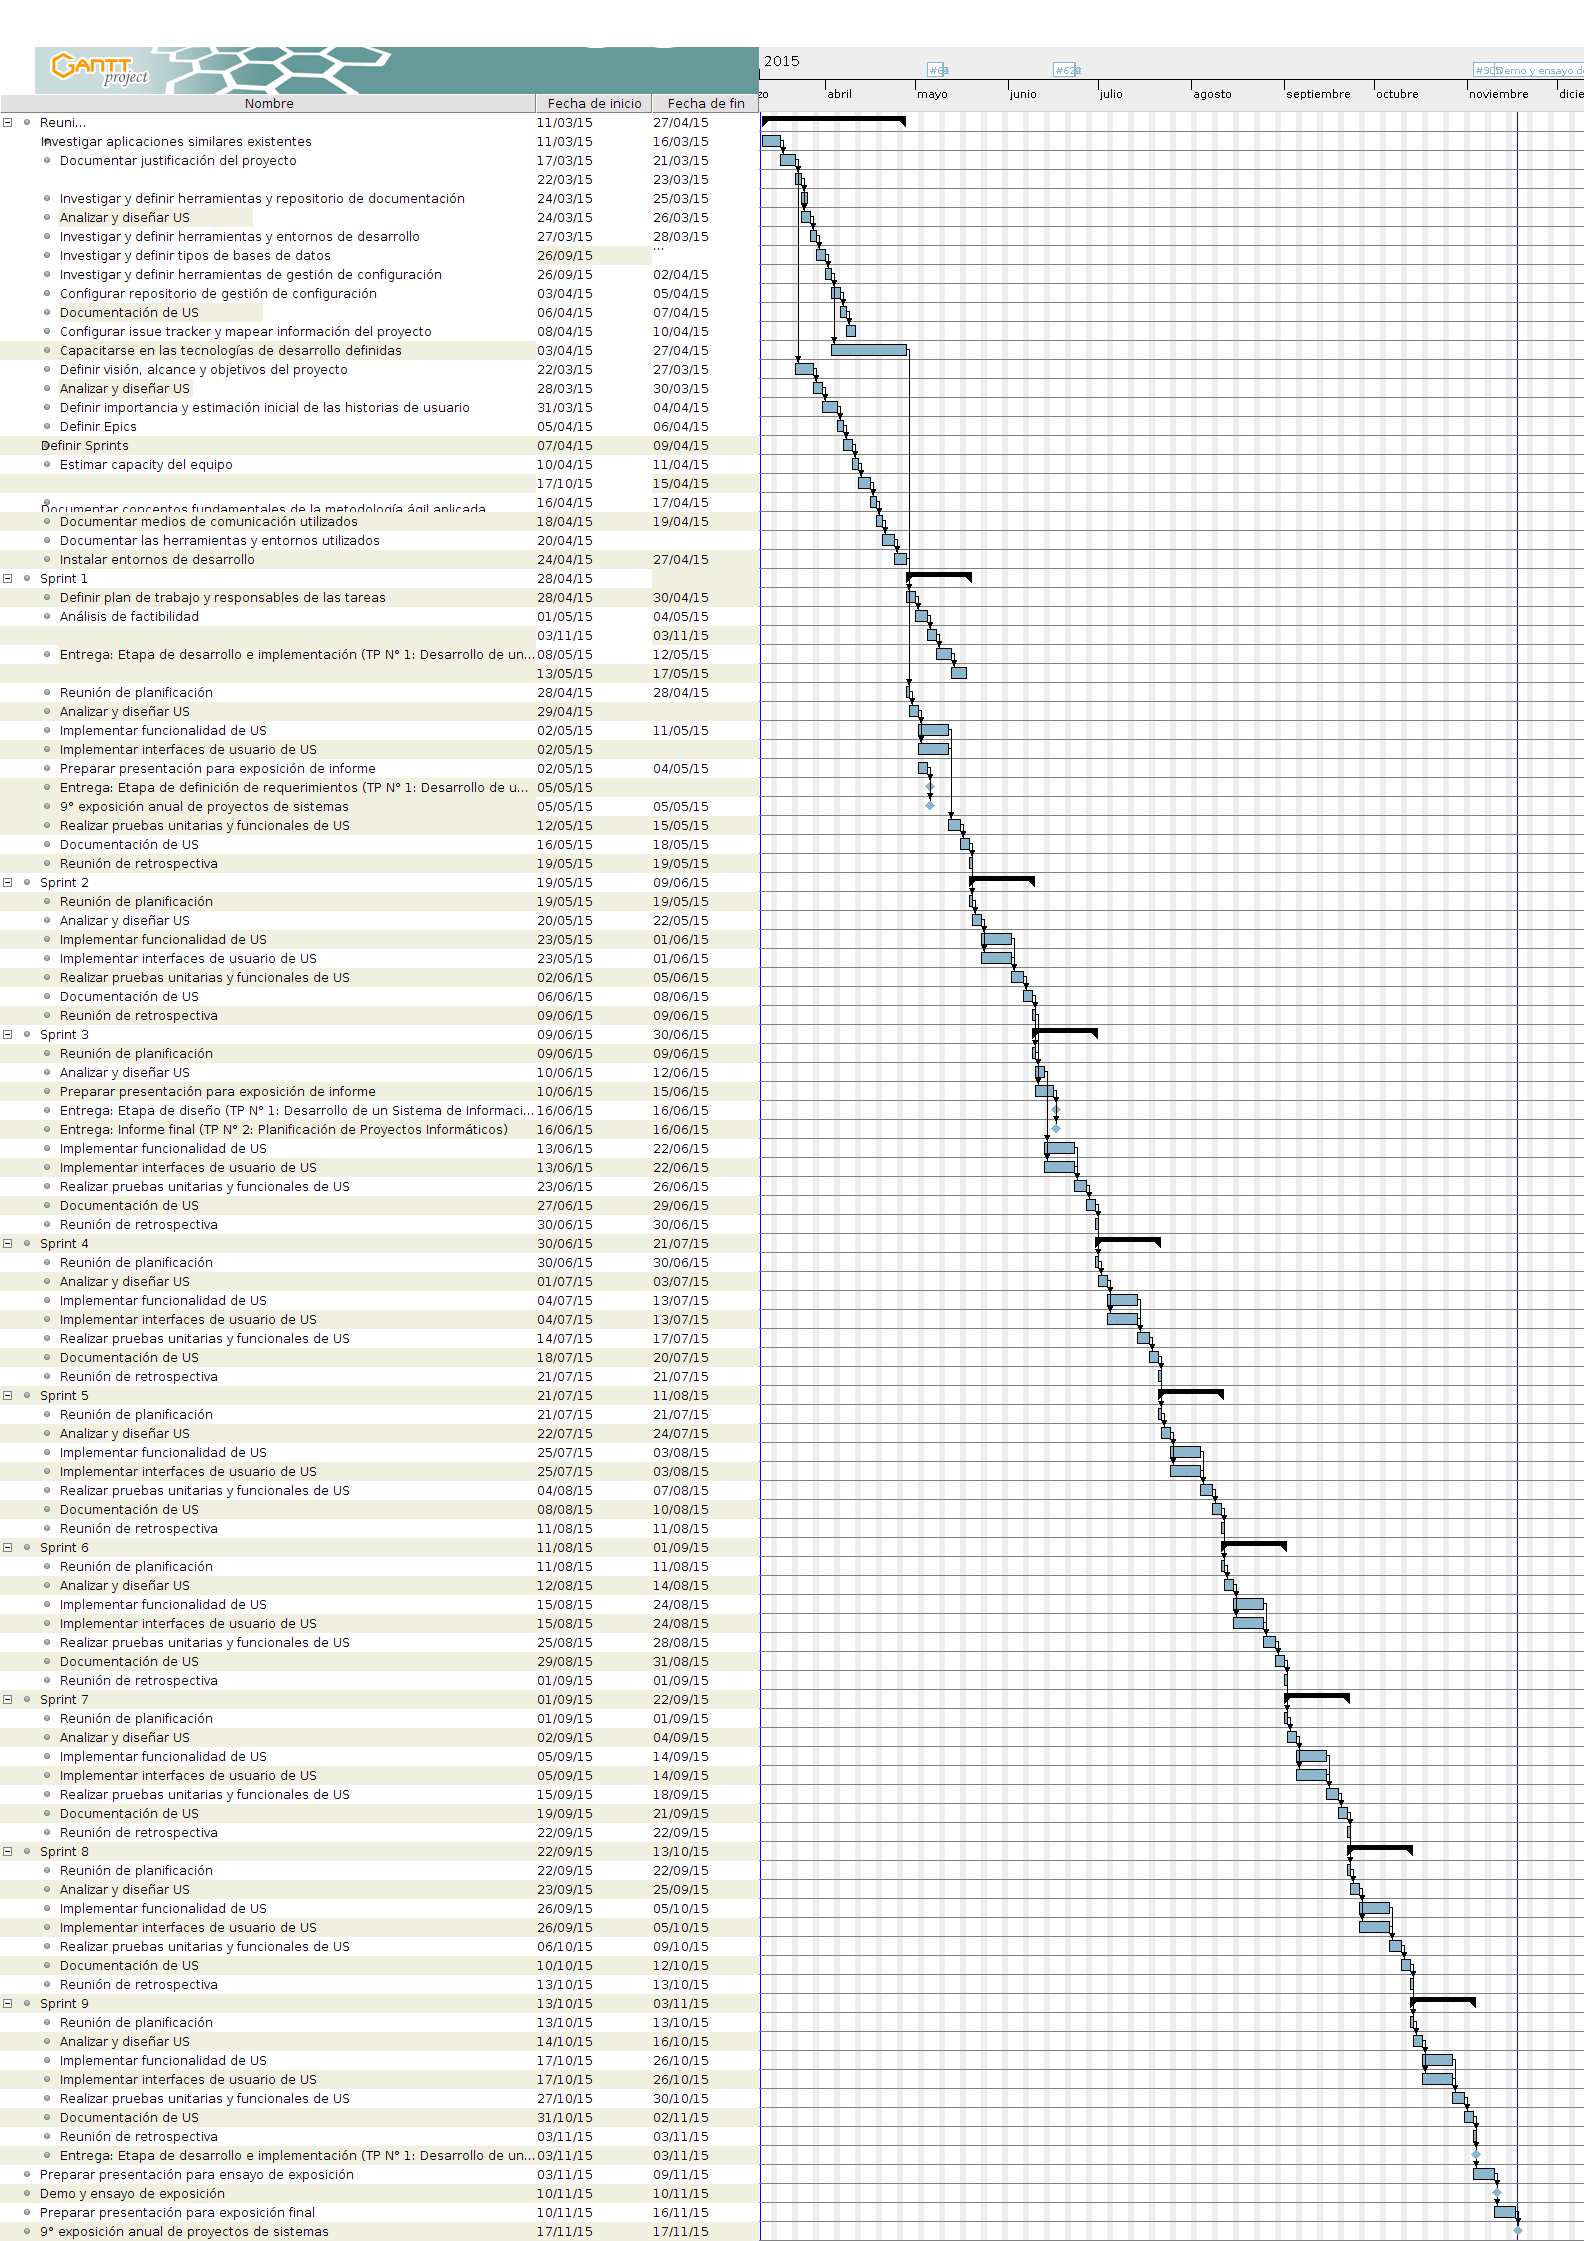
\includegraphics[width=.8\textwidth]{img/tp2_definicion/gantt}
  \caption{Diagrama de Gantt.}
  \label{imagenGantt}
\end{figure}

\newpage

                   
    
		\paragraph{Desarrollador}
		
        El desarrollador es el encargado de programar las especificaciones asignadas, así como de realizar sus pruebas unitarias y su documentación, diseñar las interfaces de usuario y desarrollar prototipos de interfaces de usuario.
		\begin{itemize}
			\item \textbf{Funciones y responsabilidades}
            	\begin{itemize}
                    \item Es el responsable del desarrollo de la aplicación, a partir de la especificaciones y requisitos planteados.
                    \item Colaborar en la confección de manuales de usuario.
                    \item Documentar adecuadamente cada modulo de desarrollo.
				\end{itemize}
            
            \item \textbf{Perfil}
                \begin{itemize}
                    \item Práctico.
                    \item Acostumbrado a trabajar bajo presión.
                    \item Poder de interpretación para lograr el mejor entendimiento de especificaciones y requisitos.
                    \item Auto-planificación de trabajo para identificar aspectos de posible dificultad o riesgo.
                    \item Abstracción de pensamiento, para descartar o reducir detalles de la significación de un problema.
                    \item Trabajo en equipo, para tener actitud abierta, estar dispuesto a compartir conocimiento e información.
                    \item Comunicación, para reconocer que existen otros que pueden aportar información útil o a quienes necesitan ayuda.

                \end{itemize}
			{\correccionTexto                
            \item \textbf{Nivel de educación / Experiencia laboral/ Antecedentes}
                \begin{itemize}
                    \item Título universitario o terciario en programación o superior
                    \item Experiencia en desarrollo de software
                    \item Conocimiento de diseño de software
                    \item Conocimientos de base de datos
                    \item Conocimientos de Python (si aspira al puesto de Back-End)
                    \item Conocimiento de Angular (si aspira al puesto de Front-End)
                \end{itemize}
            \item Herramientas y documentos necesarios para el trabajo
            	\begin{itemize}
                    \item Manejo de herramientas de programación
                    \item Experiencia con el uso de Git
                \end{itemize}
			}                
		\end{itemize}
  
    	\paragraph{Tester-QA}  
    	          	  
        El tester es la persona encargada de especificar, desarrollar y registrar las pruebas según las especificaciones del sistema, documentando los resultados y las fallas que se detecten.
			\begin{itemize}
			    \item \textbf{Funciones y responsabilidades}
            	
                \begin{itemize}
				    \item Detectar la mayor cantidad de fallas antes de que la aplicación salga a producción.
                    \item Participar de todas las etapas del proceso de desarrollo de software, colaborando para asegurar la máxima calidad del producto.
                    \item Revisar las funcionalidades de la aplicación para corroborar su correcto funcionamiento de acuerdo a lo planificado.
				\end{itemize}
            
            \item \textbf{Perfil}
            \begin{itemize}
				\item Capacidad de abstracción y modelado para atender y simular el comportamiento del sistema bajo prueba.
                \item Facilidad de comunicación oral y escrita para interactuar con desarrolladores y usuarios.
                \item Creatividad para generar ideas e imaginar los problemas que podrían existir.
                \item Pensamiento crítico para evaluar las ideas, hacer deducciones y vincular los observado con los criterios de calidad de la empresa.
                \item Aptitudes para el trabajo en equipo, de manera de poder interactuar con los desarrolladores y otros testers, y lograr el máximo beneficio en esta interacción.
            \end{itemize}
            {\correccionTexto
            \item \textbf{Nivel de educación / Experiencia laboral/ Antecedentes}
                \begin{itemize}
                    \item Título universitario afín, 
					\item Experiencia en posiciones similares al menos 2 años,
					\item Conocimiento del ciclo de vida de un sistema software, 
					\item Conocimiento de metodologías de desarrollo de sistemas, 
					\item Conocimiento y experiencia en la implementación de 							\item estándares y normas de calidad en proyectos de sistemas, 
					\item Conocimiento de los distintos tipos de casos de prueba en un sistema.
                \end{itemize}
            \item \textbf{Herramientas y documentos necesarios para el trabajo}
            	\begin{itemize}
                    \item Experiencia previa con herramientas de issues traking,
					\item Experiencia con bases de datos, verificación con queries simples,
					\item Uso de herramientas de automatización como Selenium, SOAtest y QTP,
					\item Experiencia en el uso de herramientas de seguimiento.
                \end{itemize}
            }
			\end{itemize}    
    
    
        \paragraph{Scrum Master}
        
        El Scrum Master actúa como un filtro entre el equipo y cualquier influencia que los distraiga.
        Es el responsable del proceso Scrum, debe enseñar la metodología a cada integrante implicado en el proyecto, preocupándose de ponerla en práctica de modo que se encuentre dentro de la cultura de la organización y así entregue las ventajas previstas, asegurándose de que cada uno siga las reglas y prácticas de Scrum.
        	\begin{itemize}
			\item \textbf{Funciones y responsabilidades}
            	\begin{itemize}
				\item Respaldar al equipo ante cualquier inconveniente durante el desarrollo del proyecto.
                \item Asegurar que se está cumpliendo la metodología en todos sus aspectos.
                \item Asegurar la funcionalidad y productividad del equipo.
                \item Organizar el trabajo semanal de acuerdo a las especificaciones del Gantt y a la situación del momento.
                \item Coordinar y motivar el equipo de trabajo.
                \item Prever posibles desviaciones del proyecto (tener en mente el futuro próximo).
                \item Mediar en los conflictos interpersonales del equipo.
                \item Organizar reuniones de planificación, trabajo y control.
				\end{itemize}
             
            \item \textbf{Perfil}
            	\begin{itemize}
                    \item Excelente conocimiento de Scrum.
                    \item Amplia vocación de servicio.
                    \item Tendencia altruista.
                    \item Amplia capacidad para la resolución de problemas.
                    \item Analítico y observador.
                    \item Motivador.
                    \item Capacidad docente e instructiva.
                    \item Buen carisma para las negociaciones.
				\end{itemize}
            {\correccionTexto    
            \item \textbf{Nivel de educación / Experiencia laboral/ Antecedentes}
                \begin{itemize}
                    \item  Experiencia en el desarrollo de proyectos Scrum
					\item Conocimiento de las metodologías de desarrollo de proyectos
					\item Título universitario en el área informática o de administración
					\item Experiencia en manejo de personal
					\item Conocimiento técnico 
                \end{itemize}
            \item \textbf{Herramientas y documentos necesarios para el trabajo}
            	\begin{itemize}
                    \item Conocimiento en metodologías Scrum
                    \item Manejo de Project
                    
                \end{itemize}   
            }
			\end{itemize}
        
        
        \paragraph{Product Owner}
        
        Es el dueño del producto, y es la única persona autorizada para decidir sobre cuáles funcionalidades y características funcionales tendrá el producto.
        Es quien representa al cliente, usuarios del software y todas aquellas partes interesadas en el producto.
        	\begin{itemize}
			\item \textbf{Funciones y responsabilidades}
            	\begin{itemize}
				\item Canalizar las necesidades del negocio.
                \item Maximizar el valor para el negocio.
                \item Definir las historias de usuario (\textit{user stories}).
                \item Fijar los criterios de aceptación para cada historia.
                \item Priorizar el Backlog de producto.
                \item Definir el plan de entregables.
                \item Revisar el producto, aceptar o rechazar resultados del trabajo y adaptar sus funcionalidades.
				\end{itemize}
             
            \item \textbf{Perfil}
            	\begin{itemize}
				\item Facilidad de comunicación en las relaciones interpersonales.
                \item Excelente conocimiento de las necesidades y requerimientos del producto.
                \item Facilidad para análisis de relaciones costo/beneficio.
                \item Visión de negocios.
				\end{itemize}
                
			\end{itemize}


\subsection{Capítulo II: Organización para la ejecución del proyecto}
\subsubsection{Estructura del equipo de trabajo}

En la \textbf{Tabla \ref{equipoDeTrabajo}} se detallan las funciones principales de los miembros del equipo.
Se ha considerado a cada uno de los miembros del equipo como \textit{Product Owner}, debido a que el proyecto a desarrollar es una idea de innovación, en la cual no existe la figura de un cliente.
Por este motivo, es necesario que cada uno de los integrantes aporten ideas y definan el alcance final del sistema.

Cabe aclarar que el desglose de cada una de las funciones, a saber backend y front end, se realizarán en la etapa de diseño


\begin{table}[h]
\begin{center}
\begin{tabular}{|l|c|c|c|c|}
	\hline                      & Product Owner & Scrum Master & Desarrollador & Tester     \\
	\hline Canizo, Franco       & \checkmark    &              & \checkmark    & \checkmark \\
	\hline Manganiello, Michael & \checkmark    & \checkmark   & \checkmark    & \checkmark \\
	\hline Morales, Yanina      & \checkmark    &              & \checkmark    & \checkmark \\
	\hline Terreno, Iván        & \checkmark    &              & \checkmark    & \checkmark \\
	\hline \textbf{Total}       & \textbf{4}    & \textbf{1}   & \textbf{4}    & \textbf{4} \\
\hline
\end{tabular}
\caption{Equipo de trabajo}
\label{equipoDeTrabajo}
\end{center}
\end{table}


\subsubsection{Control y comunicación}
En este apartado se definirán los métodos utilizados para la comunicación entre integrantes y las formas de documentación elegidas para llevar a cabo el proyecto elegido.


\paragraph{Métodos de comunicación formal}

Las comunicaciones internas del equipo serán guiadas a través de la técnica \textbf{\textit{Pomodoro}}, la cual nos permite administrar el tiempo, asignando un número de minutos determinado a cada tema relevante a tratar, con descansos breves de 5 minutos.

Los temas que se verán en cada reunión se listarán utilizando el editor web \textbf{\textit{Etherpad}} para que todos los integrantes tengan la posibilidad de observar y opinar por escrito y colaborativamente.


Se utilizará \textbf{\textit{Trello}} para indicar las actividades asignadas a cada participante. \textbf{\textit{Trello}} es una plataforma de trabajo que permite indicar, de forma rápida, a través de tablero cuales son aquellas actividades que se tienen que hacer, que se están haciendo y que ya se han terminado (vea \textbf{Figura \ref{trello_tareas}}). En cada tablero  se colocan tarjetas donde se indicará la fecha de presentación o fecha fin esperada, las tarjetas permiten llevar un seguimiento detallado de la situación y mantener a todo el equipo comunicado.


    \begin{figure}
      \centering
      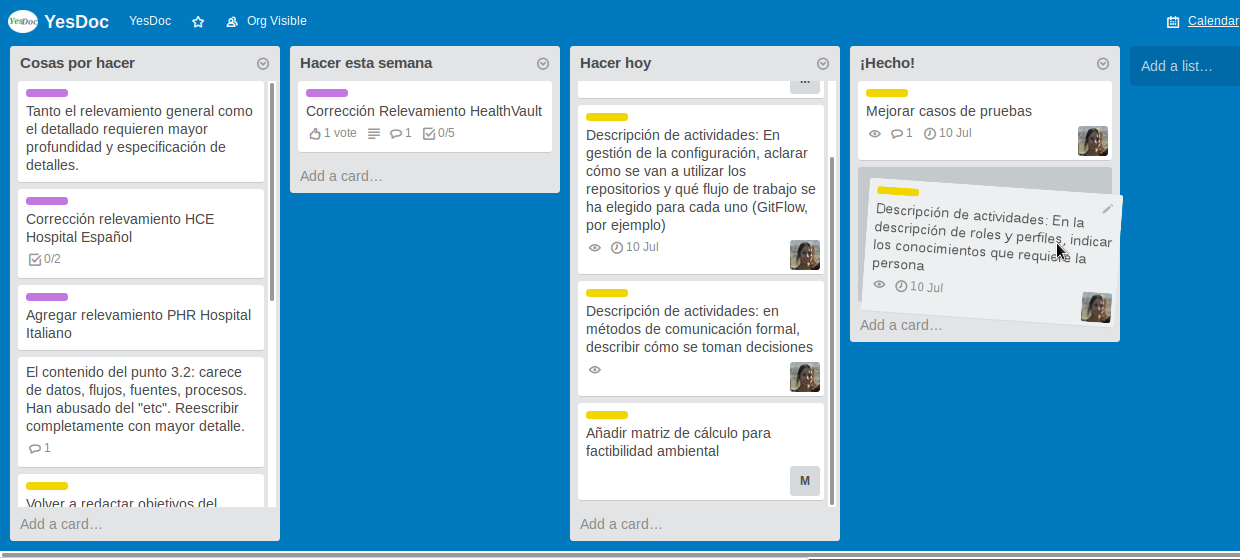
\includegraphics[width=.8\textwidth]{img/tp2_definicion/trello_tareas}
      \caption{Ejemplo de tareas en Trello.}
      \label{trello_tareas}
    \end{figure}

\paragraph{Reuniones Scrum}

La metodología Scrum lleva a que exista una retroalimentación constante que implica seguimiento y reuniones continuas, a continuación se explicará cuales serán las reuniones que se llevarán a cabo y en secciones posteriores, relacionadas al diseño, se detallará que herramientas se utilizarán en la metodología Scrum.
\begin{itemize}
	\item \textbf{Daily Scrum - Stand up meeting}:
    
    
    Haciendo uso de la técnica ágil conocida como Stand up meeting que permite  lograr el hábito en los miembros del equipo de seguir un ciclo de reuniones diarias sin tener que pasar horas cada semana en reuniones interminables, se ha determinado que  todos los días cada integrante del grupo enviará un audio a través del servicio de mensajería \textbf{\textit{Telegram}} indicando:
    \begin{itemize}
        \item Qué se ha hecho desde la última grabación.
        \item Qué se va a hacer durante ese día.
        \item Qué dificultades o impedimentos se han tenido.
    \end{itemize}
    De este modo cada uno puede saber qué es lo que falta y en que puede ayudar a otra persona. Una vez a la semana se realizará una reunión de retrospectiva para ajustar temas que necesiten ser tratados en grupo, reasignar tareas pendientes y tomar decisiones importantes que necesiten la participación de todo el equipo, la forma de tomar la decisión se detallará mas adelante en la sección de ``\textit{toma de decisiones}''. En las reuniones se documentarán los audios importantes para dejar constancia por escrito que es lo que fue realizado por cada uno de los integrantes.
    
    \textbf{La importancia del Stand up meeting}
    
    \begin{itemize}
		\item Si estas reuniones diarias son cortas, concisas y llenas de información, los miembros del equipo las apreciarán más, y no tratarán de evitarlas como lo hacen cuando se trata de reuniones tradicionales de una vez a la semana y que además duran más de tres horas.
        \item Guía al equipo por el camino hacia una mejor colaboración, fomentando a los miembros del equipo para que provean actualizaciones entre ellos, y no así al administrador del proyecto o facilitador de la reunión. Haciendo esto, el equipo comienza a ver a la “Standup Meeting” como una herramienta para coordinar su trabajo y mantenerse al tanto de lo que hacen los otros, en vez de ser un mal necesario para contestar a la pregunta ¿ya terminaste?.
	\end{itemize}
    
	\item \textbf{ Reunión de Planificación del Sprint (Sprint Planning Meeting)}

Al inicio del ciclo Sprint (cada 15 o 30 días), una “Reunión de Planificación del Sprint” se lleva a cabo.
	\begin{itemize}
	    \item Seleccionar que trabajo se hará
		\item    Preparar, con el equipo completo, el Sprint Backlog que detalla el tiempo que tomará hacer el trabajo.
		\item    Identificar y comunicar cuánto del trabajo es probable que se realice durante el actual Sprint
		\item    Ocho horas como límite
	\end{itemize}
Al final del ciclo Sprint, dos reuniones se llevaran a cabo: la “Reunión de Revisión del Sprint” y la “Retrospectiva del Sprint”
	\item \textbf{Reunión de Revisión del Sprint(Sprint Review Meeting)}
		\begin{itemize}
			\item    Revisar el trabajo que fue completado y no completado
			\item    Presentar el trabajo completado a los interesados (alias “demo”)
			\item    El trabajo incompleto no puede ser demostrado
			\item    Cuatro horas como límite
		\end{itemize}

	\item \textbf{Retrospectiva del Sprint (Sprint Retrospective)}

Después de cada sprint, se lleva a cabo una retrospectiva del sprint, en la cual todos los miembros del equipo dejan sus impresiones sobre el sprint recién superado. El propósito de la retrospectiva es realizar una mejora continua del proceso. Esta reunión tiene un tiempo fijo de cuatro horas.

	\end{itemize}

\paragraph{Métodos de comunicación informal}

Este tipo de comunicación es la resultante de las relaciones sociales que podrían aparecer entre los miembros del equipo, dando como resultado medios en los que no sólo se hable del proyecto sino de actividades relacionadas al mismo que son de interés general.
	\begin{itemize}
	\item{\textbf{Telegram}:}
	Se hará uso de este medio de comunicación informal, como principal medio de comunicación del equipo.
    \textit{Telegram} es un servicio de mensajería por internet, al igual que el conocido servicio \textit{Whatsapp}, pero con la diferencia de que permite utilizar un cliente de navegador a través de computadoras de escritorio, en cualquier navegador.
    Además, brinda un servicio de mayor seguridad y con un sistema de clientes \textit{open source} para diferentes plataformas, que se apoyan en la API de \textit{Telegram}.
    
    En \textit{Telegram} se hará uso de dos grupos: uno destinado a la comunicación estricta del proyecto y sus avances, y otro de mensajes informales que sirvan para la comunicación de novedades tecnológicas y recomendaciones.
    
	\item{\textbf{Mensaje de texto instantáneo}:}
    En algunas ocasiones, será necesario utilizar la mensajería tradicional para avisos de urgencia.
	\end{itemize}


\paragraph{Control de avance del equipo}

Una vez a la semana, se harán reuniones cortas que permitirán decidir los temas a tratar a lo largo de la semana y decidir cuáles serán los nuevos temas que va a desarrollar cada integrante del equipo.
En los casos en los que haya que trabajar en desarrollos de informes reducidos, se utilizará \textbf{\textit{Overleaf}} como editor colaborativo en línea de \LaTeX; y, una vez que se da por finalizado un informe, se añadirá a los repositorios correspondientes de documentación, para fusionarlo con los documentos ya existentes.

Esto permitirá agilizar los tiempos, llevar un control detallado de los avances y ver el resultado final y completo del documento en el que están trabajando todos los integrantes.

\LaTeX\ es un sistema de composición de texto plano, que además de brindarnos una alta calidad tipográfica nos permite aprovechar al máximo el versionado de la documentación. 
    
\paragraph{Toma de decisiones}

La elección de distintas alternativas se realizará con decisión por consenso.
Para determinar que decisión llevar a cabo se darán 15 minutos para un relevamiento general de las posibles alternativas y de este modo descartar a aquellas que no cumplan con nuestras necesidades, es muy probable que queden mas de una alternativas y se tenga que dar 10 minutos mas para que el grupo, en conjunto, realice un listado de ventajas y desventajas de cada una de las alternativas, siendo la alternativa seleccionada la que mas ventajas tenga, si existiese  algún integrante que no esté de acuerdo o considere que una de las ventajas tiene mayor peso que sobre otros se le dará 5 minutos para que exponga sus ideas.

Lo que se pretende con este método, en el que no siempre gana la mayoría, es seleccionar la opción mas conveniente para el equipo.





\subsubsection{Gestión de configuración}

Para asegurar la calidad y tener un control en tiempo real de los cambios, avances y novedades, se utilizarán diferentes repositorios con características distintas, hosteados en \textit{GitHub} y en \textit{Bitbucket}.

El manejo de distintos repositorios nos facilitará el mantenimiento del sistema, proporcionando una imagen detallada en cada etapa del desarrollo. 
Además la naturaleza distribuida de Git permite mucha más flexibilidad en la manera de colaborar en proyectos, cada desarrollador es potencialmente tanto un nodo como un repositorio --es decir, cada desarrollador puede tanto contribuir a otros repositorios, como servir de repositorio público sobre el que otros desarrolladores pueden basar su trabajo y contribuir a él. La manera como se relacionan los distintos usuarios para colaborar entre sí en la consecución de los objetivos del proyecto definen el \textit{\textbf{flujo de trabajo de un sistema de control de versiones}}.
  
Para este proyecto se ha elegido trabajar con \textbf{\textit{Flujo de trabajo del Gestor-de-Integraciones}}, el cuál nos permite mayor flexibilidad al trabajar de forma remota.  El proceso funciona de la siguiente manera (ver Figura \ref{git_integracion}):
	\begin{enumerate}
		\item    La persona gestora del proyecto (actualmente los cuatro integrantes del grupo) envían (push) a su repositorio público (repositorio principal).
		\item    Una persona que desea contribuir, realizará un fork de dicho repositorio y hará algunos cambios (cada uno de los cuatro integrantes hará un fork del repositorio principal).
		\item    La persona colaboradora envia (push) a su propia copia pública.
		\item    Esta persona colaboradora envía un pull request al repositorio principal solicitándo se integren los cambios.
		\item    Los gestores revisan el código y si no hay errores aceptan los cambios.
	\end{enumerate}
\begin{figure}
  \centering
  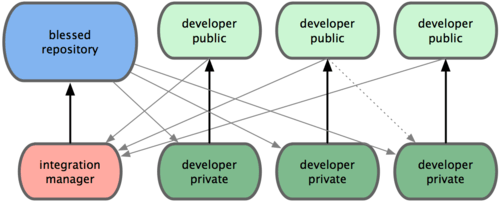
\includegraphics[width=.8\textwidth]{img/tp2_definicion/git_integracion}
  \caption{Flujo de trabajo Gestor-de-Integración.}
  \label{git_integracion}
\end{figure}

A continuación se detallarán los repositorios a utilizar, cabe aclarar que todos utilizarán el flujo de trabajo antes descrito.
	\begin{itemize}
	\item \textbf{Repositorios de desarrollo}:
	Se utilizará más de un repositorio de desarrollo, todos hosteados en \textit{GitHub} y con licencia \textit{GPLv3}.
    La diferencia entre estos repositorios yace en la plataforma o capa de la arquitectura a desarrollar.
    
    En un primer momento, se tendrá un repositorio para la capa de servicio (\textit{back-end}) del sistema, uno para la interfaz de usuario web, y otro para la aplicación móvil.

	\item \textbf{Repositorio de documentación}:
    Este repositorio de \textit{GitHub} será destinado a todo lo referido a la documentación del proyecto.

	\item \textbf{Repositorio para la wiki personal del proyecto}:
	Este repositorio, hosteado en \textit{GitHub}, se utilizará para aquella información relevante que se desea recalcar sobre las tecnologías de desarrollo y las herramientas usadas para la documentación.
    Se hará uso de una estructura jerárquica de directorios, para separar el contenido de cada tema relevante.
    
    Es la base de conocimiento del equipo, y concentrará toda la información y referencias importantes que faciliten la capacitación propia y de terceros con respecto a las tecnologías y herramientas utilizadas durante todo el proyecto.

	\item \textbf{Repositorio de documentación privada}:
	Este repositorio será privado y hosteado en \textit{Bitbucket}, y en el mismo se almacenará aquella información delicada relacionada al proyecto.

    \item \textbf{Servicio de alojamiento de archivos}:
    Para el manejo de imágenes y fotos se hará uso del servicio de \textbf{\textit{Mega}}, el cual provee 50 GB de almacenamiento.
    También provee la posibilidad de ser sincronizado en las máquinas de escritorio y accedido mediante aplicaciones móviles.
    Cuenta además con un visor de imágenes que facilita la consulta de las mismas desde el sitio web.
	\end{itemize}


\subsubsection{Herramientas a utilizar en el desarrollo}
A continuación, se presenta los resultados de las investigaciones de las diferentes herramientas de desarrollo que soportarán el desarrollo del proyecto.

\paragraph{Integración continua}

	Una herramienta de \textbf{integración continua} permite que se lleven a cabo a cabo integraciones automáticas (compilación y ejecución de pruebas unitarias y de integración) del código, para poder detectar errores antes de que los cambios pasen a formar parte de la rama de trabajo principal del proyecto.

En el caso de este proyecto, permitirá controlar cada \textit{pull request} de los repositorios de desarrollo, ejecutando la totalidad de las pruebas diseñadas, antes de que éstas sean aceptadas e integradas.

En la \textbf{Figura \ref{comparativaIC}} se detalla en forma gráfica la comparación efectuada de las siguientes herramientas de integración continua relevadas:
\begin{itemize}
    \item CircleCI
    \item Codeship
    \item Drone.io
    \item Shippable
    \item Travis CI
\end{itemize}


\begin{figure}
  \centering
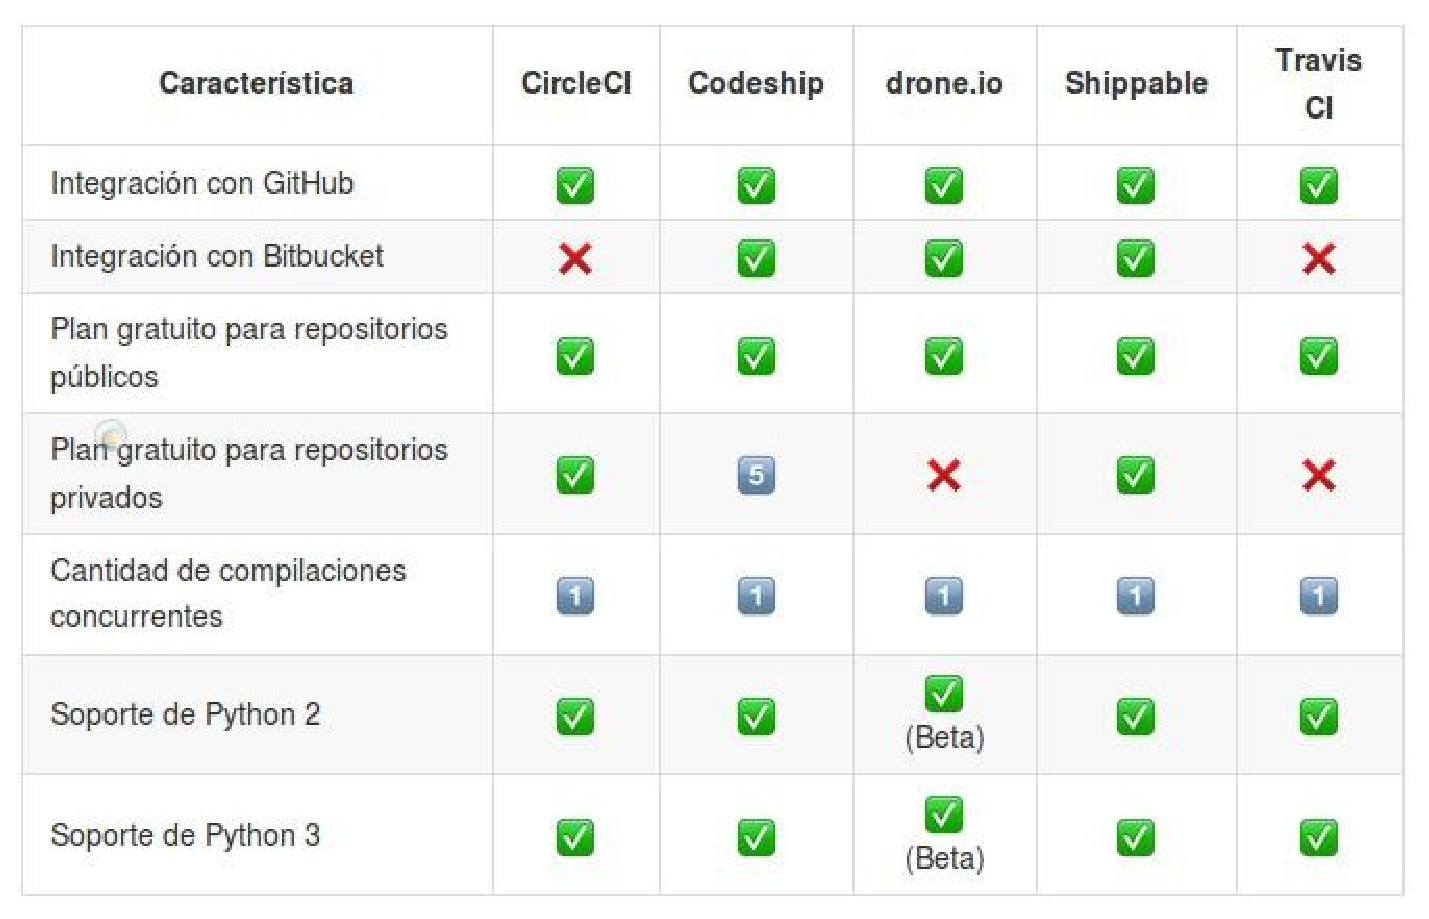
\includegraphics[width=1\textwidth]{img/tp2_definicion/integContinua}
  \caption{Cuadro comparativo de \textit{integración continua}.}
  \label{comparativaIC}
\end{figure}

\textbf{Elección}: Shippable

\textbf{Justificación}:
La integración con \textit{Bitbucket} además de \textit{GitHub}, la posibilidad de integrar un número ilimitado de repositorios privados en forma gratuita, y el soporte extendido para las versiones 2 y 3 de \textit{Python}, posicionan a \textbf{Shippable} como principal opción para llevar a cabo la integración continua del proyecto.


\paragraph{Front-end}

El \textbf{front-end} es la parte del software que interactúa con el usuario.
Este concepto es necesario para mantener el sistema correctamente desacoplado y poder añadir nuevas interfaces de acceso al sistema sin duplicar esfuerzos a nivel de servicio y funcionalidad del sistema.

Es importante hacer hincapié en una navegación simple e intuitiva para el usuario, que permita el uso del sistema sin la necesidad de una capacitación prolongada sobre las funcionalidades que se brindan.


\textbf{Lenguajes y herramientas relevadas}:

\begin{itemize}
\item \textbf{AJAX}: 
\textit{Asynchronous JavaScript And XML}.
Es un paradigma que necesita de un lenguaje de scripting, como por ejemplo \textit{JavaScript}, para detectar las acciones del usuario y modificar los respectivos elementos.
Realiza peticiones al servidor. 

\item \textbf{jQuery}:
Librería de \textit{JavaScript}, que provee funcionalidades ligeras y sencillas de alto nivel.
Permite incrustar la lógica en la misma página (acceder y modificar un elemento) sin recurrir al servidor.

\item \textbf{AngularJS}:
Librería de \textit{JavaScript} (se acerca más a un framework de aplicaciones web).
Marca una serie de normas y hábitos en la programación, gracias al patrón \textit{MVC}.
Añade a \textit{jQuery} (usa \textit{jqLite}) una serie de mecanismos por los cuales extender el HTML, y ahorrar líneas de código.

\item \textbf{HTML5}:
Añade a HTML nuevos elementos semánticos, como etiquetas y características de \textit{JavaScript}.

\item \textbf{CSS3}:
Brinda propiedades que permiten definir estilos y animaciones.
\end{itemize}

\textbf{Comparativa entre \textit{jQuery} y \textit{AngularJS}}:

Son dos librerías distintas, que muchas veces se pueden complementar (aunque no es recomendable).

\textit{AngularJS} está destinada a aplicaciones web complejas, más parecidas a las aplicaciones de escritorio, con uso muy intensivo de \textit{JavaScript}.
En cambio, \textit{jQuery} está destinada a sitos web en los que \textit{JavaScript} tiene poco peso, y se está limitado a crear interfaces de usuario dinámicas o pequeños comportamientos interactivos.

\textbf{Conclusión}:
Para poder explotar por completo \textit{AJAX}, \textit{jQuery}, \textit{AngularJS} y los elementos de \textit{HTML5} es necesario conocer de \textit{JavaScript}, y así poder darle a la página mayor interacción con el usuario. 
Para facilitar el uso de \textit{JavaScript}, se hará uso de \textbf{AngularJS}, ya que permite escribir código con un mayor nivel de desacoplamiento y abstracción.


\paragraph{Desarrollo móvil}

Hoy en día, el desarrollo móvil adquiere importancia por el alcance masivo que provee.
Sin embargo, a la hora de desarrollar para esta plataforma, se pueden encontrar sistemas que implementan interfaces distintas, y que se tienen que añadir capaz(como por ejemplo el navegador web), encima de estas interfaces para alcanzar cierta uniformidad.

Esta reseña tiene por idea principal explicar brevemente cada una de las alternativas más importantes del desarrollo móvil:

\begin{itemize}
\item \textbf{Native app}:
Son aplicaciones diseñadas y codificadas para tipos de dispositivos específicos, pudiendo acceder a las características propias como cámara, acelerómetro, etc.
Por ejemplo, las aplicaciones de iPhone están escritas en \textit{Swift} u \textit{Objetive-C}; las aplicaciones de Android, en \textit{Java}.
Se obtienen de las diferentes \textit{App Stores}.

\item \textbf{Web app}:
Son aplicaciones web, por lo que están preparadas para trabajar en navegadores web móviles.
Cuando se ingresa a cualquier página web desde el teléfono, que ofrece un mínimo de \textit{User Experience}, hablamos de \textit{Web App}.
Dentro de este enfoque de desarrollo podemos hacer otra clasificación, en: 
\begin{itemize}
    \item Webs con diseño responsive: es una única página web, que adapta su contenido según el dispositivo que realiza la solicitud.
    \item Web apps propiamente dichas: son múltiples páginas web; por ejemplo, una para dispositivos móviles y otra diferente para computadoras de escritorio.
\end{itemize}

\item \textbf{Hybrid app}:
Son en parte \textit{Native apps} y en parte \textit{Web apps}.
Como las aplicaciones nativas, se obtienen de las \textit{App Stores} y pueden acceder a ciertas características de los dispositivos, como cámara, acelerómetro, etc.
Al igual que las aplicaciones web, se basan en HTML que se renderiza en el navegador, con el detalle de que el navegador está embebido dentro de la aplicación.

\end{itemize}


\textbf{Comparación}:
En la \textbf{Figura \ref{appMobile}} se puede observar la comparación gráfica de las distintas posibilidades de desarrollo móvil.

\begin{figure}
  \centering
  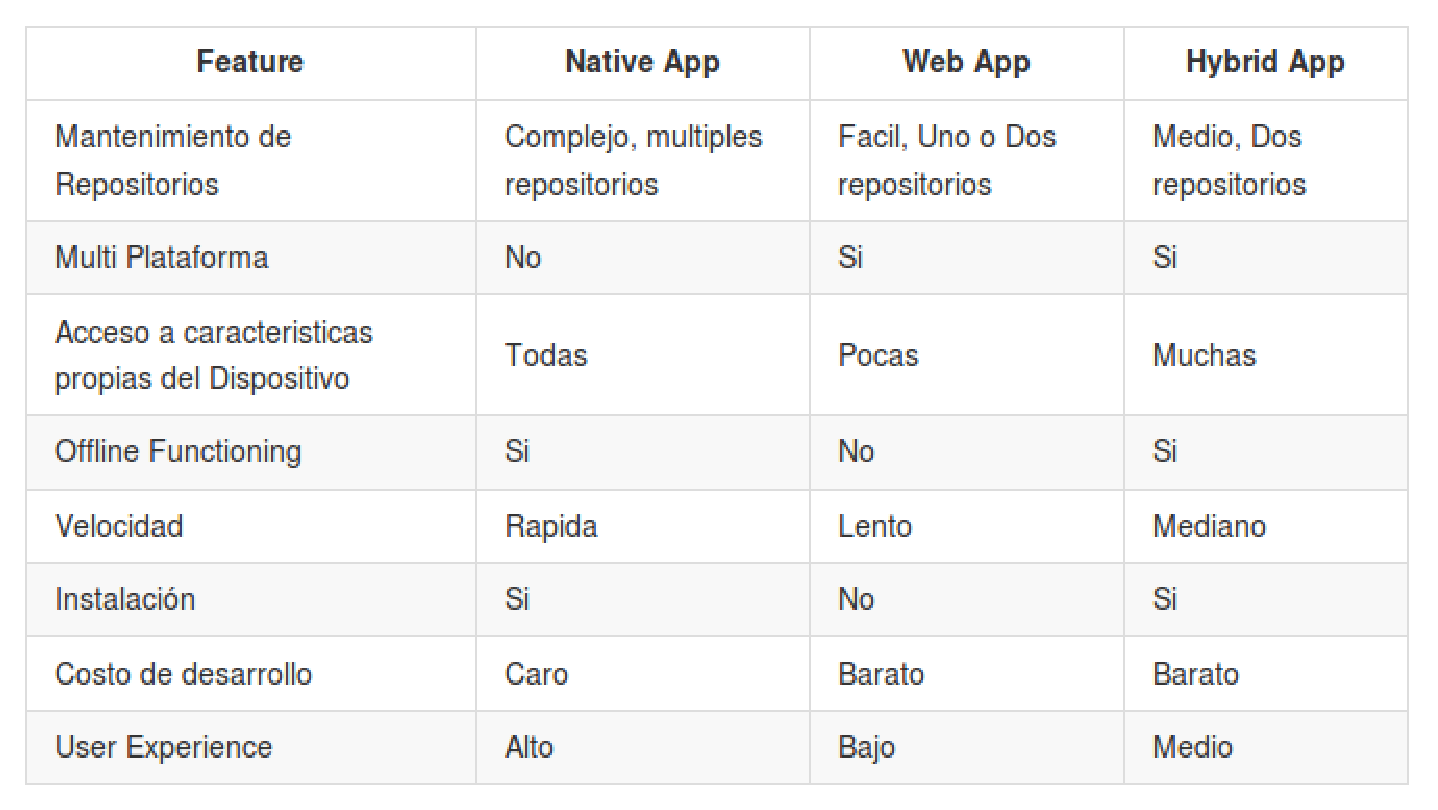
\includegraphics[width=1\textwidth]{img/tp2_definicion/appMobile}
  \caption{Cuadro comparativo de \textit{desarrollo móvil}.}
  \label{appMobile}
\end{figure}

\textbf{Conclusión}:

Se hará uso de aplicaciones híbridas (\textit{Hybrid apps}), utilizando como framework a \textbf{Ionic} ya que ofrece al proyecto la máxima flexibilidad y agilidad a la hora de desarrollar para los distintos dispositivos.
\textit{Ionic} cuenta con una comunidad activa que ofrece un mayor y mejor soporte a la hora de detectar y resolver problemas.




% \newpage



% \section{CAPITULO III: Factibilidad.  }
% \subsubsection{Definición y descripción de recursos para cada una de las actividades. }
% \subsubsection{Diagrama de recursos. }
% \subsubsection{Análisis de factibilidad. }
% \subsubsection{Costos desagregados por recursos (personal, tecnología) con periodicidad mensual. }
% \subsubsection{Análisis de riesgos. }
% \subsubsection{Análisis del impacto ambiental. } 





